\section{Task Definition}
\begin{figure*}
    \centering
    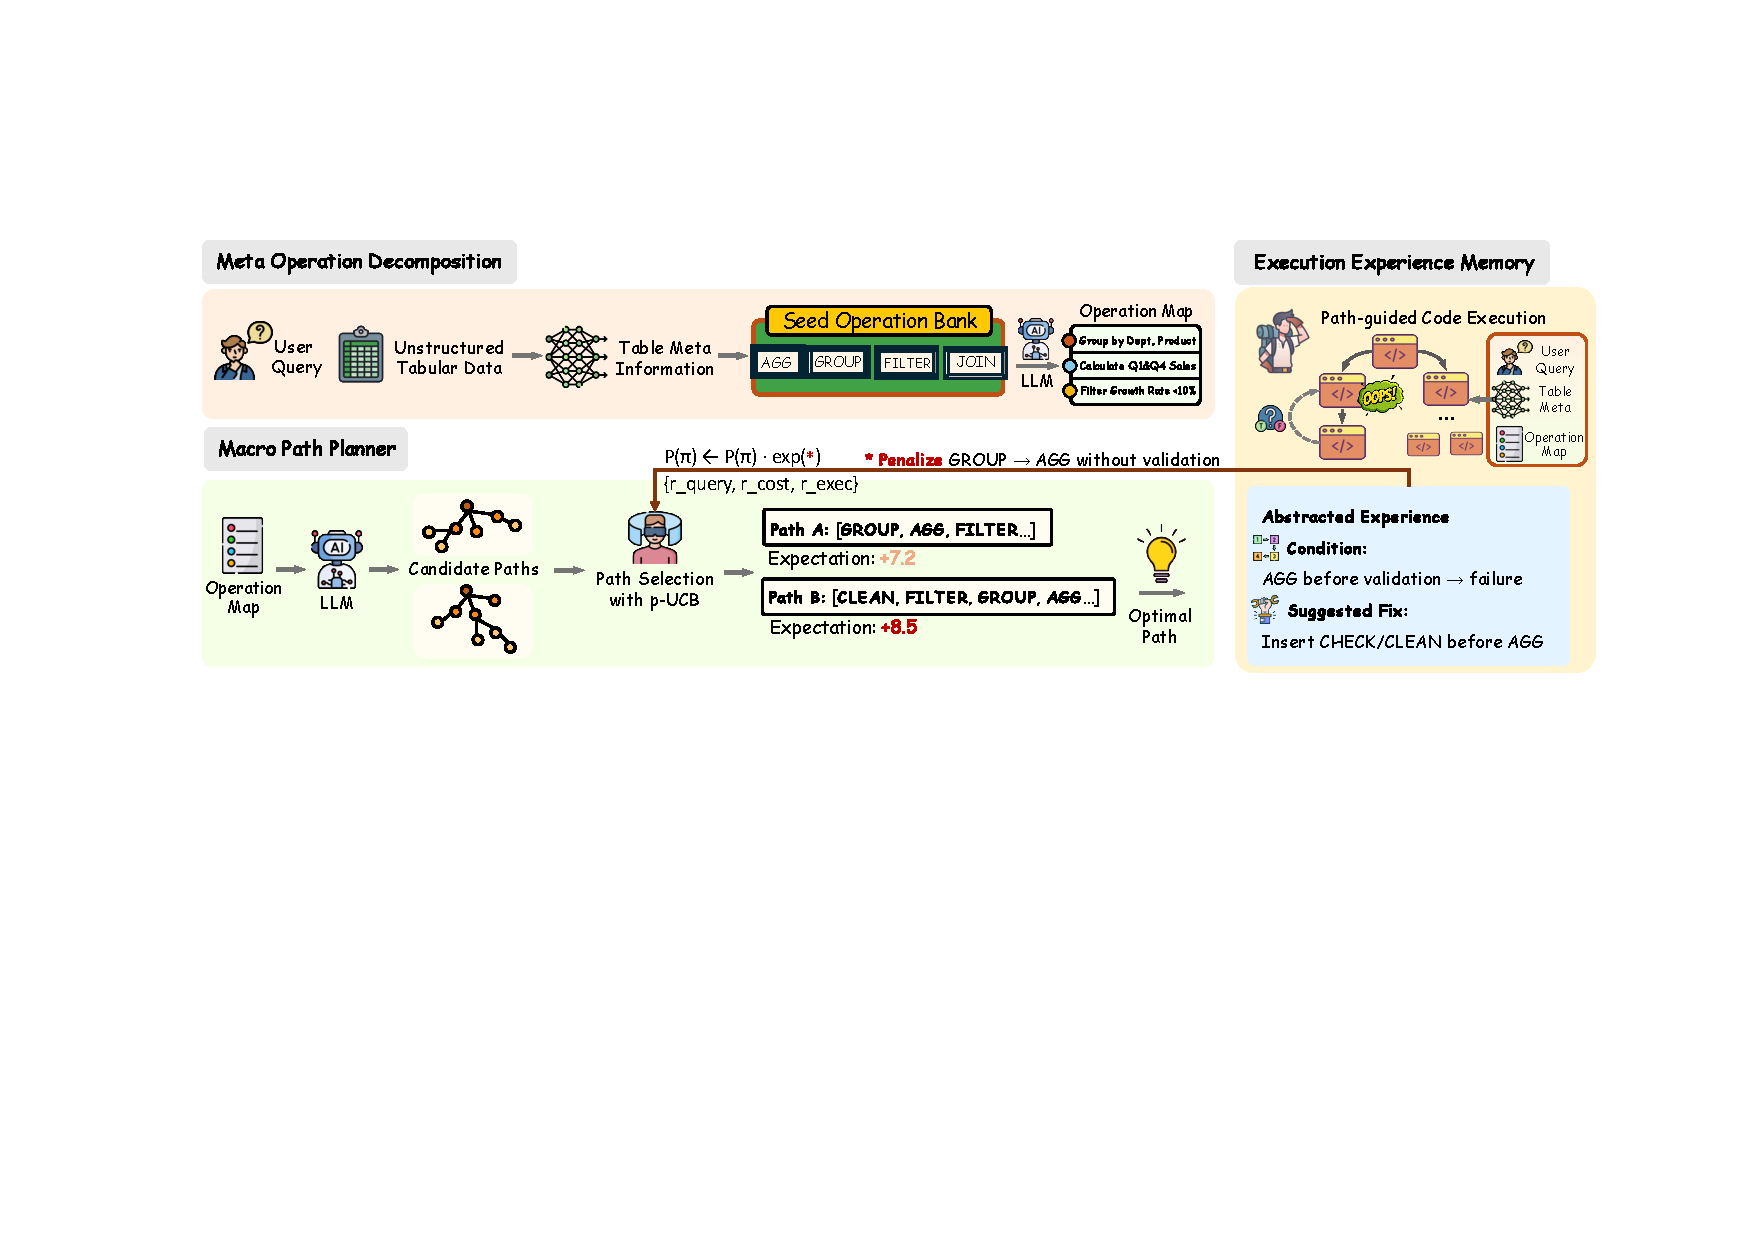
\includegraphics[width=0.95\linewidth]{resources/figure1.pdf}
    \caption{A sketched overview for our proposed Deep Tabular Research framework for complex unstructured tabular reasoning. DTR decomposes analytical intent into meta operations, plans executable macro paths via expectation-guided search, and executes them with an experience-aware memory that records structured execution feedback and updates planning policies across iterations.}
    \label{fig:figure1}
\end{figure*}
Deep Tabular Research (DTR) generalizes the problem of answering complex, multi-step analytical queries over non-canonical tables. Formally, a DTR task is defined by the tuple $(\mathcal{T}, \mathcal{Q}, \mathcal{E}, \mathcal{Y})$, representing the tabular domain, the query space, the execution environment, and the output space, respectively.

\fbox{\parbox{\linewidth}{
Let $T \in \mathcal{T}$ be an unstructured table with flexible schemas, $T$ may contain hierarchical headers, bidirectional row-column spans, and implicit semantic relations. Given a natural language query $q \in \mathcal{Q}$ that requires long-horizon reasoning (e.g., trend analysis, cross-region comparison, or recursive aggregation), the task is to produce a response $y \in \mathcal{Y}$ that is both factually accurate and computationally grounded.}}
\subsection{Execution-Grounded Paradigm}
Unlike traditional TableQA with a pure linguistic mapping $f(q, T) \to y$, DTR defines reasoning as an interactive exploration within an execution environment $\mathcal{E}$, where the agent incrementally executes operations and adapts its strategies.

\begin{itemize}[leftmargin=*]\item \textbf{Latent Structural State:} The true semantic structure of $T$ (e.g., the exact scope of a hierarchical header) is latent and must be inferred through interaction since raw data rarely presents explicit hierarchical dependencies.\item \textbf{Analytical Trajectory:} To resolve $q$, a sequence of atomic analytical actions $\mathbf{a} = (a_1, a_2, \dots, a_H)$ must be performed. Each $a_i$ represents a data-level transformation that maps an input data state to an intermediate result $o_i$.\item \textbf{State Transition:} The reasoning state at step $t$ is defined as $\mathcal{S}_t = \{q, T, (a_1, o_1), \dots, (a_{t-1}, o_{t-1})\}$. The objective is to find a trajectory of actions such that the final outcome $o_H$ supports the generation of correct output $y$.\end{itemize}

% \subsection{Core Challenges}

% The complexity of DTR stems from three intrinsic properties of the task: \textbf{Structural Ambiguity:} Because the table $T$ is unstructured, the validity of any action $a_t$ is highly sensitive to the model's interpretation of headers and cell alignments. A single misaligned index can render the entire subsequent trajectory invalid. \textbf{Long-Horizon Dependency:} DTR tasks often exhibit deep causal chains where the parameters of action $a_t$ depend on the specific output $o_{t-1}$ of the preceding step. This requires the model to maintain consistency over extended reasoning horizons. \textbf{Observational Uncertainty:} In an unstructured setting, the environment $\mathcal{E}$ may return unexpected outcomes—such as empty sets or runtime exceptions—even for logically sound queries. A successful DTR process must therefore account for the potential need to revise and backtrack based on these observations.The goal of a DTR system is to navigate these challenges to produce a verifiable and robust analytical result $y$ across diverse and irregular tabular layouts.
